%%%%%%%%%%%%%%%%%%%%%%%%%%%%%%%%%%%%%%%%%
% Beamer Presentation
% LaTeX Template
% Version 1.0 (10/11/12)
%
% This template has been downloaded from:
% http://www.LaTeXTemplates.com
%
% License:
% CC BY-NC-SA 3.0 (http://creativecommons.org/licenses/by-nc-sa/3.0/)
%
%%%%%%%%%%%%%%%%%%%%%%%%%%%%%%%%%%%%%%%%%

%----------------------------------------------------------------------------------------
%	PACKAGES AND THEMES
%----------------------------------------------------------------------------------------

\documentclass{beamer}

\mode<presentation> {

% The Beamer class comes with a number of default slide themes
% which change the colors and layouts of slides. Below this is a list
% of all the themes, uncomment each in turn to see what they look like.

%\usetheme{default}
%\usetheme{AnnArbor}
%\usetheme{Antibes}
%\usetheme{Bergen}
%\usetheme{Berkeley}
%\usetheme{Berlin}
%\usetheme{Boadilla}
%\usetheme{CambridgeUS}
%\usetheme{Copenhagen}
%\usetheme{Darmstadt}
%\usetheme{Dresden}
%\usetheme{Frankfurt}
%\usetheme{Goettingen}
%\usetheme{Hannover}
%\usetheme{Ilmenau}
%\usetheme{JuanLesPins}
%\usetheme{Luebeck}
\usetheme{Madrid}
%\usetheme{Malmoe}
%\usetheme{Marburg}
%\usetheme{Montpellier}
%\usetheme{PaloAlto}
%\usetheme{Pittsburgh}
%\usetheme{Rochester}
%\usetheme{Singapore}
%\usetheme{Szeged}
%\usetheme{Warsaw}

% As well as themes, the Beamer class has a number of color themes
% for any slide theme. Uncomment each of these in turn to see how it
% changes the colors of your current slide theme.

%\usecolortheme{albatross}
%\usecolortheme{beaver}
%\usecolortheme{beetle}
%\usecolortheme{crane}
%\usecolortheme{dolphin}
%\usecolortheme{dove}
%\usecolortheme{fly}
%\usecolortheme{lily}
%\usecolortheme{orchid}
%\usecolortheme{rose}
%\usecolortheme{seagull}
%\usecolortheme{seahorse}
%\usecolortheme{whale}
%\usecolortheme{wolverine}

%\setbeamertemplate{footline} % To remove the footer line in all slides uncomment this line
%\setbeamertemplate{footline}[page number] % To replace the footer line in all slides with a simple slide count uncomment this line

%\setbeamertemplate{navigation symbols}{} % To remove the navigation symbols from the bottom of all slides uncomment this line
}

\usepackage{graphicx} % Allows including images
\usepackage{booktabs} % Allows the use of \toprule, \midrule and \bottomrule in tables
\usepackage[utf8]{inputenc}


\setbeamertemplate{caption}{\raggedright\insertcaption\par}

\graphicspath{ {images/} }

%----------------------------------------------------------------------------------------
%	TITLE PAGE
%----------------------------------------------------------------------------------------

\title[BRKGA - BL - TOP]{Biased Random Key Genetic Algorithm con B\'usqueda Local para el Team Orienteering Problem} % The short title appears at the bottom of every slide, the full title is only on the title page

\author{Alejandro Lix Klett} % Your name
\institute[UBA] % Your institution as it will appear on the bottom of every slide, may be shorthand to save space
{
Directora: Prof. Dra. Irene Loiseau\\ 
\medskip
Departamento de Computaci\'on\\ % Your institution for the title page
%\textit{john@smith.com} % Your email address
}
\date{\today} % Date, can be changed to a custom date

\begin{document}

\begin{frame}
\titlepage % Print the title page as the first slide
\end{frame}

\begin{frame}[allowframebreaks]
\frametitle{Contenido} % Table of contents slide, comment this block out to remove it

\tableofcontents[sections={1-2}]
    \framebreak
  \tableofcontents[sections={3-6}]
%\tableofcontents % Throughout your presentation, if you choose to use \section{} and \subsection{} commands, these will automatically be printed on this slide as an overview of your presentation
\end{frame}

%----------------------------------------------------------------------------------------
%	PRESENTATION SLIDES
%----------------------------------------------------------------------------------------

%------------------------------------------------

\section{El Problema}
\subsection{Orienteering Problem} % Sections can be created in order to organize your presentation into discrete blocks, all sections and subsections are automatically printed in the table of contents as an overview of the talk
%------------------------------------------------

%\subsection{Historia} % A subsection can be created just before a set of slides with a common theme to further break down your presentation into chunks
%\subsection{Descripci\'on}

\begin{frame}
\frametitle{Orienteering Problem}

\begin{itemize}
    \item Orientaci\'on es un deporte originario de Escandinavia
    \pause
    \item Cada jugador comienza en un punto de control y debe visitar tantos otros puntos de control como le sea posible dentro de un tiempo límite preespecificado. 
    \pause
    \item Cada punto de control tiene un puntaje.
    \pause
    \item Cada punto de control puede ser visitado una sola vez a lo sumo.
    \pause
    \item El objetivo es maximizar el puntaje total.
    \pause
    \item Este problema se conoce como Orienteering Problem (OP). El OP es NP-Hard como demostraron Golden, Levy y Vohra.
\end{itemize}

\end{frame}

%%%%%%%%%%%%%%%%%%%%%%%%%%%%%%%%%%%%%%%%%%%%%%

\subsection{Team Orienteering Problem}
\begin{frame}
\frametitle{Team Orienteering Problem}

\begin{itemize}
    \item Hay \textit{M} clientes, cada uno tiene un beneficio $b_i$ y una coordenada en el plano.
    \pause
    \item Los puntos de salida y llegada tienen beneficio cero
    \pause    
    \item Hay \textit{N} veh\'iculos
    \pause
    \item El beneficio de los clientes solo puede ser recolectado una vez.
    \pause
    \item El objetivo es maximizar la sumatoria de los beneficios recolectados de todos los vehículos.
    \pause
    \item Como TOP contiene a OP, es al menos tan dif\'icil.
\end{itemize}

\end{frame}

%%%%%%%%%%%%%%%%%%%%%%%%%%%%%%%%%%%%%%%%%%%%%%

\subsection{Ejemplo de solución de TOP}

\begin{frame}
\frametitle{Instancia p2.2.k del benchmark de Tsiligirides}

La instancia tiene dos vehículos con un $d_{max}$ = 22,50. Hay 19 clientes además de los puntos de salida y llegada.% La imagen muestra la solución óptima del problema.

\begin{figure}[h]
	\centering
	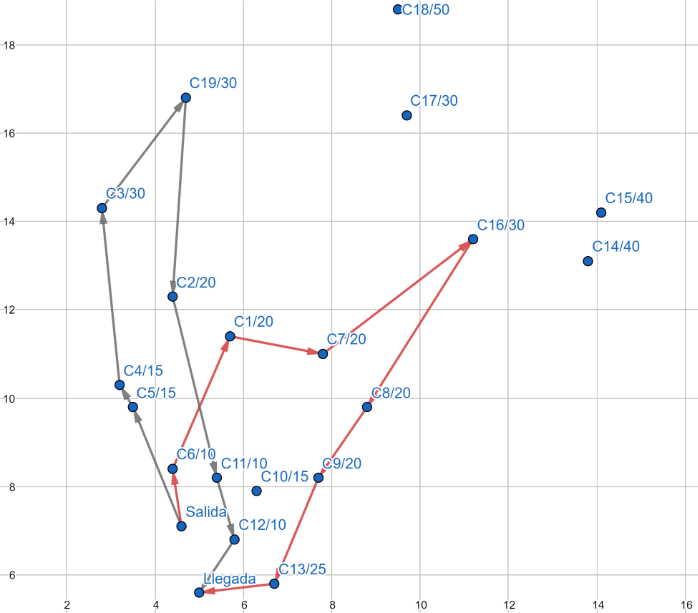
\includegraphics[width=7.5cm]{400cropped}
	\label{fig:400cropped}
\end{figure}


\end{frame}

%%%%%%%%%%%%%%%%%%%%%%%%%%%%%%%%%%%%%%%%%%%%%%

\subsection{Aplicaciones}

\begin{frame}
\frametitle{Aplicaciones}

\begin{itemize}
	\item El deporte de orientación de equipo explicado anteriormente (que también se puede jugar en equipo).
	\pause
	\item Tsiligirides hace mención del caso del Travelling Sales Person (TSP) sin tiempo suficiente para visitar a todos los clientes y que conoce de antemano el valor aproximado de las ventas que realizará en cada ciudad.
	\pause
	\item El reclutamiento de jugadores de fútbol americano universitario descrito en el trabajo de Butt y Cavalier. Los representante de las pequeñas ligas deben visitar la máxima cantidad de escuelas en un radio de 100 km, de antemano saben que no llegan a visitar a todas las escuelas.
\end{itemize}

\end{frame}

%%%%%%%%%%%%%%%%%%%%%%%%%%%%%%%%%%%%%%%%%%%%%%


\begin{frame}
\frametitle{Aplicaciones}

\begin{itemize}
	\item El problema de entrega de combustible con múltiples vehículos descrito en el trabajo Golden, Levy y Vohra. Una flota de camiones debe entregar combustible a una gran cantidad de clientes diariamente. El suministro de combustible del cliente debe mantenerse en un nivel adecuado en todo momento. Los desabastecimientos son costosos y deben evitarse en tanto sea posible.
\end{itemize}

\end{frame}

%%%%%%%%%%%%%%%%%%%%%%%%%%%%%%%%%%%%%%%%%%%%%%

\section{Metaheurísticas}
\subsection{Descripción}

\begin{frame}
\frametitle{Metaheurísticas}

\begin{itemize}
    \item Son métodos diseñados para encontrar buenas soluciones, en un tiempo razonable, a problemas de optimización combinatoria en general.
    \pause
    \item Las metaheurísticas son estrategias de alto nivel que guían una heurística específica del problema a resolver para mejorar su perfomance.
    \pause
\end{itemize}

Caracter\'isticas:

\begin{itemize}
    \item Son estrategias que gu\'ian procesos de búsqueda.
    \pause
    \item Sus conceptos se pueden describir con un gran nivel de abstracción. No son para un problema específico.
    \pause
    \item En muchos casos son algoritmos no-determin\'isticos.
    \pause
    \item Sus desarrollos y diseños suelen estar motivados por comportamientos naturales.
    \pause
    \item No garantizan que una soluci\'on \'optima sea encontrada.
    \pause
    \item Las t\'ecnicas metaheur\'isticas van desde algoritmos simples de b\'usqueda local a complejos procesos de aprendizaje.
\end{itemize}

\end{frame}

%%%%%%%%%%%%%%%%%%%%%%%%%%%%%%%%%%%%%%%%%%%%%%

\begin{frame}
\frametitle{Metaheurísticas}

Algunas técnicas:

\begin{itemize}
    \item Simulated Annealing
    \pause
    \item Búsqueda Tabú
    \pause
    \item Algoritmos evolutivos
    \pause
    \item Colonia de hormigas
    \pause
    \item Variable Neighborhood Search
    \pause
    \item Iterated Local Search
    \pause
    \item Etc
\end{itemize}

\end{frame}

%%%%%%%%%%%%%%%%%%%%%%%%%%%%%%%%%%%%%%%%%%%%%%

\subsection{Algoritmos genéticos (GA)}

\begin{frame}
\frametitle{Algoritmos genéticos (GA)}

\begin{itemize}
    \item Motivados en el concepto de supervivencia del más apto.
    \pause
    \item Los algoritmos genéticos manejan un conjunto de individuos.
    \pause
    \item Cada individuo es un cromosoma que codifica una solución.
    \pause
    \item Cada cromosoma tiene asociado un nivel de condición física que está correlacionado con el correspondiente valor de la función objetivo de la solución que codifica.
    \pause
    \item En cada generación se crea una nueva población con individuos provenientes de tres fuentes distintas: crossover, elites y mutantes.
\end{itemize}

\end{frame}

%%%%%%%%%%%%%%%%%%%%%%%%%%%%%%%%%%%%%%%%%%%%%%

\subsection{Random Key Genetic Algorithm (RKGA)}

\begin{frame}
\frametitle{Random Key Genetic Algorithm (RKGA)}

\begin{itemize}
    \item Los individuos son representados por un vector de números reales en el intervalo [0, 1].
    \pause
    \item La población inicial es generada al azar.
    \pause
    \item El decodificador es el responsable de convertir un cromosoma en una solución válida del problema.
    \pause
    \item En cada iteración se toman los mejores individuos y pasan directamente a la siguiente generación (elites).
    \pause
    \item La mayoría de los individuos de la nueva generación se genera cruzando dos individuos de la generación actual (crossover).
    \pause
    \item Un porcentaje muy bajo de los nuevos individuos es generado al azar, para escapar de mínimos locales (mutantes).
\end{itemize}

\end{frame}

%%%%%%%%%%%%%%%%%%%%%%%%%%%%%%%%%%%%%%%%%%%%%%

\subsection{Biased Random Key Genetic Algorithm (BRKGA)}

\begin{frame}
\frametitle{Biased Random Key Genetic Algorithm (BRKGA)}

\begin{itemize}
    \item Cada individuo se genera combinando un elemento seleccionado al azar del conjunto de elite y el otro de la conjunto no elite.
    \pause
    \item Parameterized Uniform Crossover. La probabilidad de que se trasmita el alelo del padre de elite es mayor que la del padre de no elite.
\end{itemize}

\end{frame}

%%%%%%%%%%%%%%%%%%%%%%%%%%%%%%%%%%%%%%%%%%%%%%

\section{Algoritmo Propuesto}

\begin{frame}
\frametitle{Diagrama de flujo del BRKGA}

\begin{figure}[h]
	\centering
	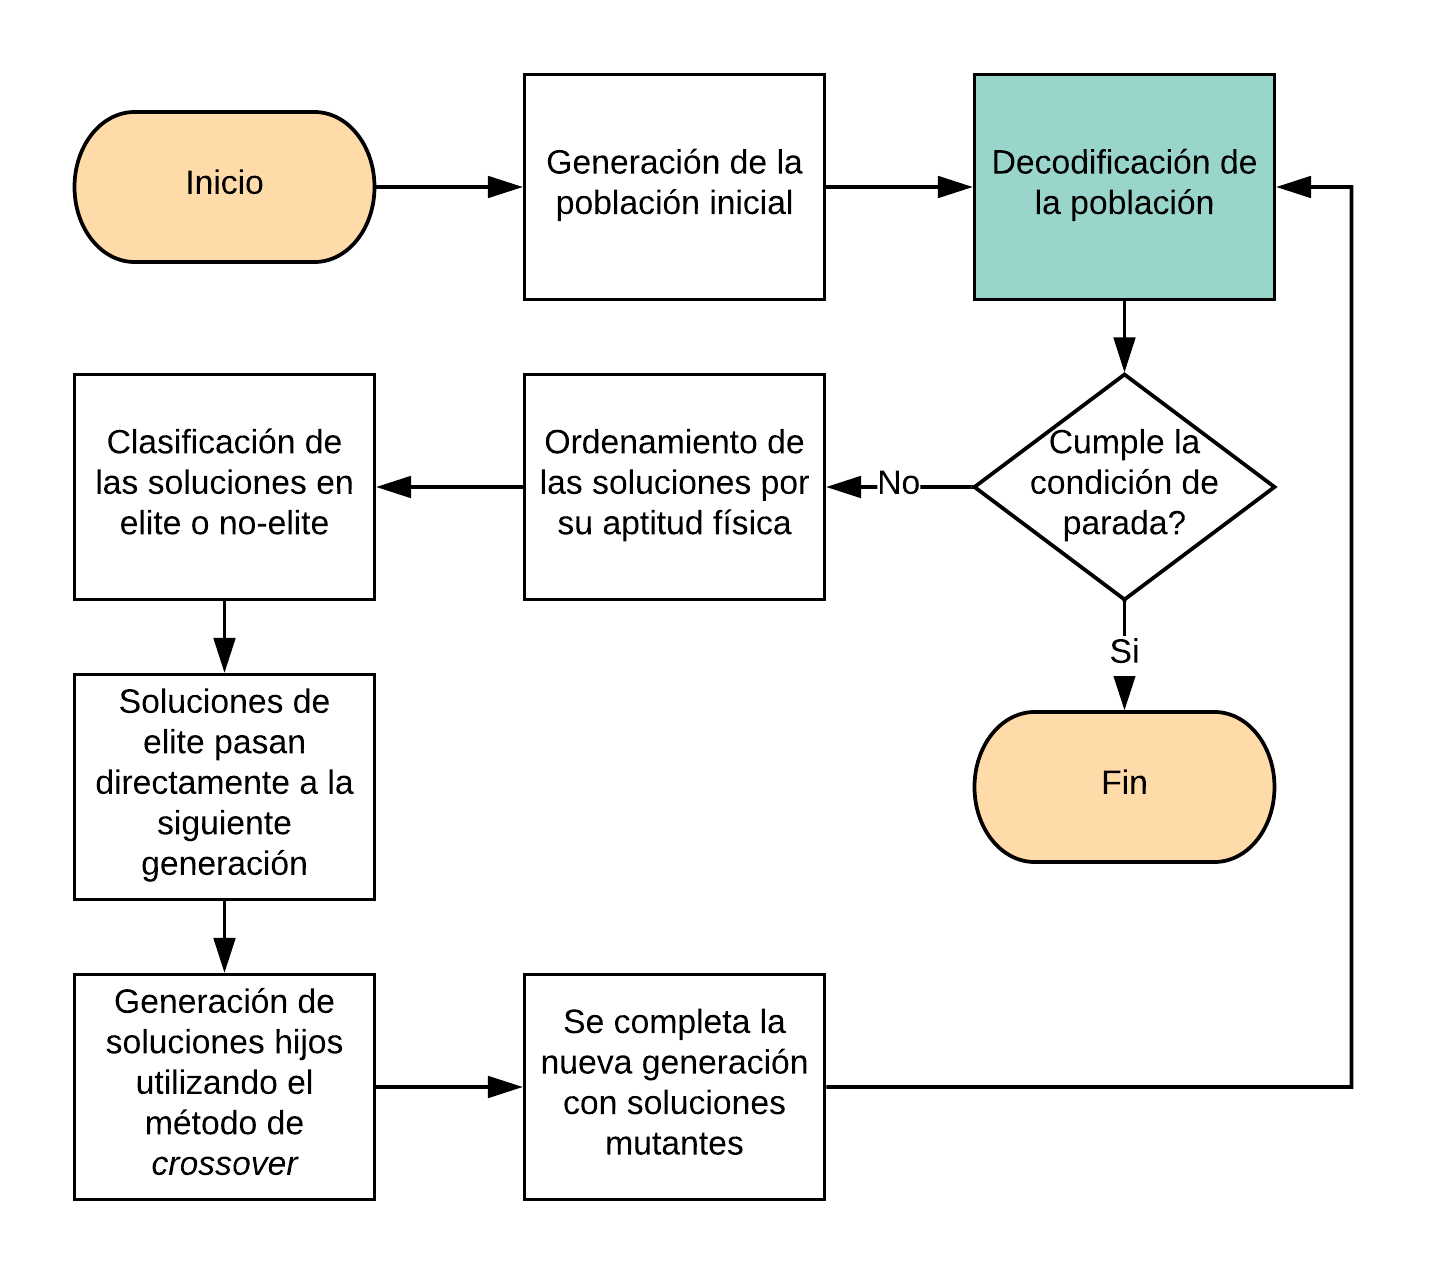
\includegraphics[width=8cm]{BRKGA_Flow_Chart_Base}
	\label{fig:BRKGA_Flow_Chart_Base}
\end{figure}

\end{frame}

%%%%%%%%%%%%%%%%%%%%%%%%%%%%%%%%%%%%%%%%%%%%%%

\subsection{Generación de la población inicial}

\begin{frame}
\frametitle{Generación de la población inicial}

\begin{itemize}
    \item Se crea una cantidad de vectores de enteros aleatorios igual a la cantidad de soluciones por generación que se desea.
    \pause
    \item Los vectores tienen un tamaño igual a la cantidad de clientes de la instancia.
    \pause
    \item Cada entero aleatorio del vector esta asociado a un identificador de cliente.
    \pause
\end{itemize}

\begin{figure}[h]
	\caption{Ejemplo de un nuevo vector de enteros aleatorios.}
	\centering
	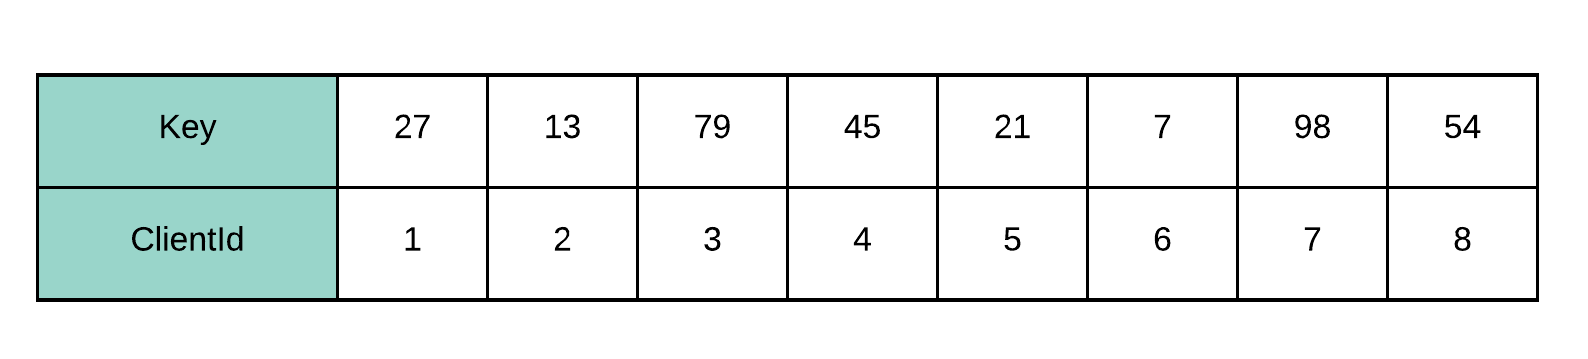
\includegraphics[width=9cm]{RandomKeysInicializado}
	\label{fig:RandomKeysInicializado}
\end{figure}

\end{frame}

%%%%%%%%%%%%%%%%%%%%%%%%%%%%%%%%%%%%%%%%%%%%%%

\subsection{Decodificadores}

\begin{frame}
\frametitle{Decodificación de los vectores en soluciones válidas del problema}

\begin{itemize}
    \item Se ordena el vector de enteros aleatorios por el valor de la clave aleatoria de forma ascendente.
    \pause
\end{itemize}

\begin{figure}[h]
	\caption{Ejemplo del vector de enteros aleatorios ordenado.}
	\centering
	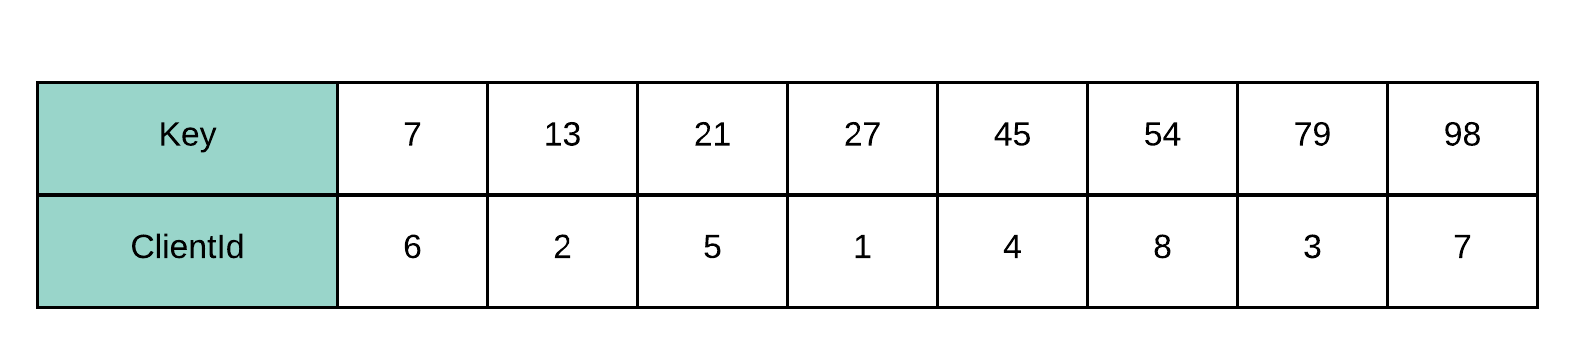
\includegraphics[width=9cm]{RandomKeysOrdenado}
	\label{fig:RandomKeysOrdenado}
\end{figure}

\begin{itemize}
    \pause
    \item Implementé dos decodificadores cada uno con su estrategia para generar soluciones.
    \pause
    \item Ambos decodificadores generan una solución válida del problema a partir de un vector de enteros aleatorios ordenado.
\end{itemize}

\end{frame}

%%%%%%%%%%%%%%%%%%%%%%%%%%%%%%%%%%%%%%%%%%%%%%

\begin{frame}
\frametitle{Decodificador simple}

\begin{itemize}
    \item Los vehículos están ordenados de forma ascendente según su identificador.
    \pause
    \item Toma el primer cliente e intenta agregarlo en la ruta del primer vehículo disponible.
    \pause
    \item Si logra insertarlo repite el proceso con el siguiente cliente para el mismo vehículo.
    \pause
    \item Si no lo logra, considera que la ruta del vehículo actual esta completa e intenta agregar el mismo cliente en el siguiente vehículo disponible.
    \pause
    \item Repite hasta completar la ruta de todos los vehículos disponibles.
    \pause
\end{itemize}

\begin{figure}[h]
	\caption{Ejemplo de la solución generada por el decodificador simple}
	\centering
	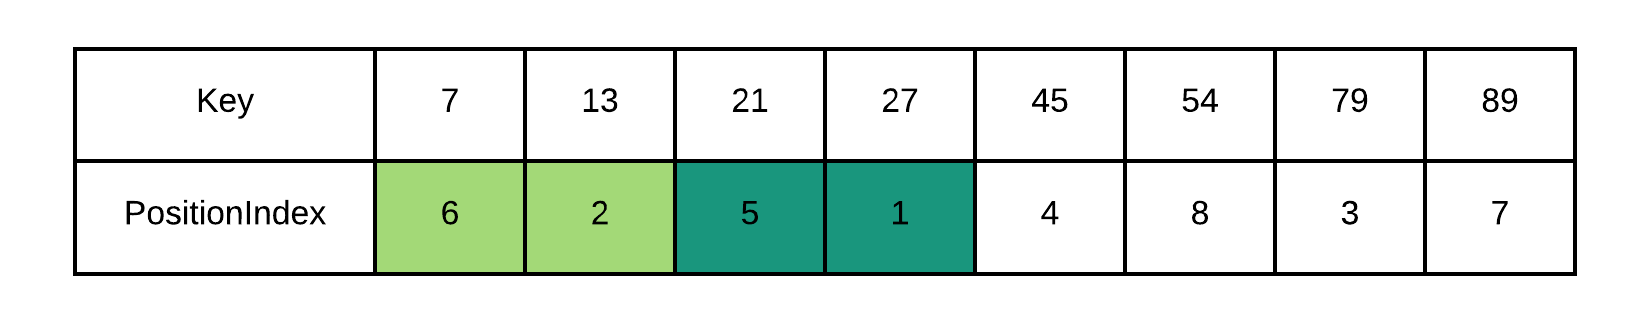
\includegraphics[width=9cm]{DistribucionClientesDecoSimple}
	\label{fig:DistribucionClientesDecoSimple}
\end{figure}

\end{frame}

%%%%%%%%%%%%%%%%%%%%%%%%%%%%%%%%%%%%%%%%%%%%%%

\begin{frame}
\frametitle{Decodificador goloso}

\begin{itemize}
    \item Se diferencia del decodificador simple en el momento en que encuentra un cliente que no entra en la ruta del vehículo actual.
    \pause
    \item En vez de pasar al siguiente vehículo, prueba con el siguiente cliente.
    \pause
    \item Por lo tanto, por cada vehículo prueba todos los clientes en el orden dado.
    \pause
    \item No prueba con los clientes que ya fueron asignados a otro vehículo.
    \pause
\end{itemize}

\begin{figure}[h]
	\caption{Ejemplo de la solución generada por el decodificador goloso}
	\centering
	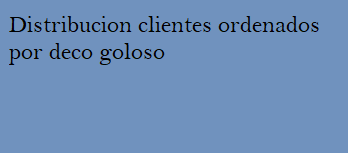
\includegraphics[width=9cm]{DistribucionClientesDecoGoloso}
	\label{fig:DistribucionClientesDecoGoloso}
\end{figure}

\end{frame}

%%%%%%%%%%%%%%%%%%%%%%%%%%%%%%%%%%%%%%%%%%%%%%

\begin{frame}
\frametitle{Descripción de las columnas de resultados}

\begin{itemize}
	\item \textbf{$Instancia$}: Nombre de la instancia utilizada.
	\item \textbf{$N/V/D$}: Cantidad de \textbf{N}odos / Cantidad de \textbf{V}ehículos / \textbf{D}istancia máxima de la ruta del vehículo
	\item \textbf{$T_{avg}$}: El \textbf{T}iempo promedio en milisegundos de la ejecución del algoritmo para la instancia mencionada sobre $n$ ejecuciones.
	\item \textbf{$D$}: El \textbf{D}ecodificador utilizado.
\end{itemize}

\end{frame}

%%%%%%%%%%%%%%%%%%%%%%%%%%%%%%%%%%%%%%%%%%%%%%

\begin{frame}
\frametitle{Descripción de las columnas de resultados}

\begin{itemize}
	\item \textbf{$B_{max}$}: El \textbf{B}eneficio máximo que obtuve para la instancia mencionada sobre $n$ ejecuciones.
	\item \textbf{$B_{min}$}: El \textbf{B}eneficio mínimo que obtuve para la instancia mencionada sobre $n$ ejecuciones.
	\item \textbf{$B_{avg}$}: El \textbf{B}eneficio promedio que obtuve para la instancia mencionada sobre $n$ ejecuciones.
	\item \textbf{$i_{eMax}$}: Indice de efectividad máximo. $i_{eMax}=B_{max}/Best$
	\item \textbf{$i_{eAvg}$}: Indice de efectividad promedio. $i_{eAvg}=B_{avg}/Best$
	\item \textbf{$Best$}: Máximo beneficio obtenido por algún trabajo previo sobre la misma instancia mencionada.
\end{itemize}

\end{frame}

%%%%%%%%%%%%%%%%%%%%%%%%%%%%%%%%%%%%%%%%%%%%%%

\begin{frame}
\frametitle{Comparación entre decodificadores}

\begin{itemize}
    \item Se realizó una prueba para comparar los tiempos de ejecución y aptitud de las soluciones generadas por ambos decodificadores.
    \pause
    \item Se crearon 200 vectores de enteros aleatorios y se decodificaron utilizando ambos decodificadores.
    \pause
\end{itemize}

\begin{table}
\begin{center}
\begin{tabular}{ |c|c|c|c|c|c|c|c|c| } 
\hline
Instancia & N/V/D & D & $B_{min}$ & $B_{avg}$ & $B_{max}$ & $i_{eAvg}$ & $Best$ \\
\hline
p2.2.k & 21/2/22.50 & S & 50 & 101 & 170 & 0.37 & 275 \\
p2.2.k & 21/2/22.50 & G & 105 & 166 & 230 & 0.60 & 275 \\
p2.3.g & 21/3/10.70 & S & 45 & 84 & 140 & 0.58 & 145 \\
p2.3.g & 21/3/10.70 & G & 90 & 122 & 145 & 0.84 & 145 \\
p5.3.x & 66/3/40.00 & S & 195 & 301 & 425 & 0.19 & 1555 \\
p5.3.x & 66/3/40.00 & G & 305 & 412 & 560 & 0.26 & 1555 \\
p7.2.e & 102/2/50.00 & S & 8 & 39 & 113 & 0.13 & 290 \\
p7.2.e & 102/2/50.00 & G & 37 & 95 & 171 & 0.33 & 290 \\
p7.4.t & 102/4/100.00 & S & 38 & 114 & 238 & 0.11 & 1077 \\
p7.4.t & 102/4/100.00 & G & 165 & 273 & 439 & 0.25 & 1077 \\
\hline
\end{tabular}
\end{center}
\label{tab:resultadosDecoSimple}
\end{table}


\end{frame}

%%%%%%%%%%%%%%%%%%%%%%%%%%%%%%%%%%%%%%%%%%%%%%

\subsection{Condición de parada}

\begin{frame}
\frametitle{Condición de parada}

\begin{itemize}
    \item Cantidad de iteraciones.
    \pause
    \item \'Ultimas X generaciónes sin que haya mejorado el beneficio de la mejor solución.
    \pause
    \item Ambas condiciones deben ser válidas a la vez para que termine el algoritmo.
\end{itemize}

\end{frame}

%%%%%%%%%%%%%%%%%%%%%%%%%%%%%%%%%%%%%%%%%%%%%%

\subsection{Evolución de la población}

\begin{frame}
\frametitle{Evolución de la población}

\begin{itemize}
    \item Se ordenan las soluciones por su aptitud física. (vectores decodificados)
    \pause
    \item Las mejores $X$ soluciones se agregan al conjunto elite y pasan directamente a la siguiente generación.
    \pause
    \item El resto de las $\#Poblacion-X$ soluciones, se agregan al conjunto no elite.
    \pause
    \item Se generan $Y$ soluciones mutantes del mismo modo que se generaron las soluciones iniciales que se agregan a la nueva generación.
    \pause
    \item Se completa la nueva generación mediante el proceso de \textit{crossover}. Proceso por el cual a partir de dos individuos se genera un tercer individuo.
\end{itemize}

\end{frame}

%%%%%%%%%%%%%%%%%%%%%%%%%%%%%%%%%%%%%%%%%%%%%%

\begin{frame}
\frametitle{Evolución de la población}

\begin{figure}[h]
	\centering
	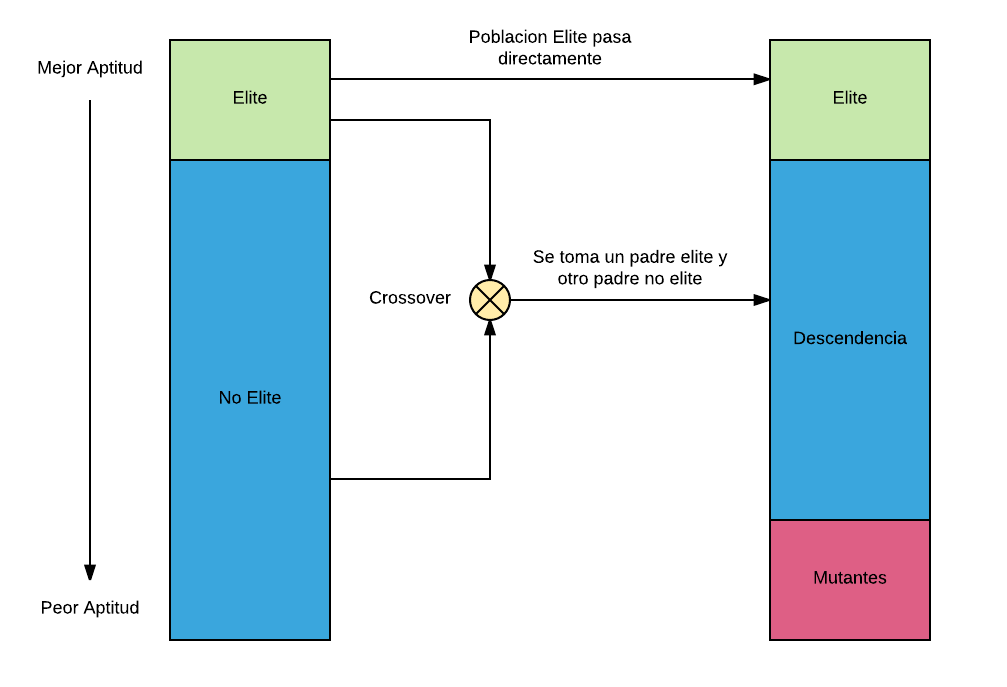
\includegraphics[width=12cm]{EvolucionPoblacion}
	\label{fig:EvolucionPoblacion}
\end{figure}

\end{frame}

%%%%%%%%%%%%%%%%%%%%%%%%%%%%%%%%%%%%%%%%%%%%%%

\subsection{Crossover}

\begin{frame}
\frametitle{Crossover}

\begin{itemize}
    \item Se toma un cromosoma del conjunto de elite y otro del conjunto de no elite.
    \pause
    \item Se crea un vector de números reales al azar en el intervalo [0, 1] del mismo tamaño que los cromosomas.
    \pause
    \item Si el valor en la posición $i$ del vector de números reales es menor a $\rho_e$, el cromosoma hijo hereda el alelo de la posición $i$ del padre elite. En caso contrario el cromosoma hijo hereda el alelo de la posición $i$ del padre no elite.
    \pause
    \item El valor de $\rho_e$ suele ser $0.70$, favoreciendo los alelos del cromosoma elite.
\end{itemize}

\end{frame}

%%%%%%%%%%%%%%%%%%%%%%%%%%%%%%%%%%%%%%%%%%%%%%

\begin{frame}
\frametitle{Crossover}

\begin{figure}[h]
	\centering
	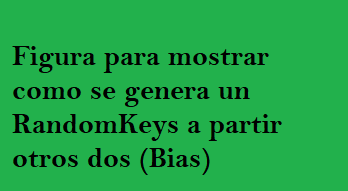
\includegraphics[width=12cm]{BiasCrossover}
	\label{fig:BiasCrossover}
\end{figure}

\end{frame}

%%%%%%%%%%%%%%%%%%%%%%%%%%%%%%%%%%%%%%%%%%%%%%

\subsection{Hash de un individuo}

\begin{frame}
\frametitle{Hash de un individuo}

\begin{itemize}
    \item Dos individuos son iguales si representan la misma solución.
    \pause
    \item Tener individuos repetidos en la población reduce el dominio de soluciones exploradas.
    \pause
    \item Tener individuos repetidos en la población genera cálculos repetidos.
    \pause
    \item Un individuo se inserta en la población si no existe algún individuo en la población con el mismo valor de hash.
    \pause
    \item Se implementaron dos formas de calcular el hash de un individuo.
    \pause
    \item La primer forma que implemente calcula el hash sin conocer el problema que se esta resolviendo, luego mantiene la evolución de la población independiente del problema que se esta resolviendo.
    \pause
    \item La segunda forma de calcular es óptima detectando repetidos y requiere conocer el problema que se esta resolviendo.
\end{itemize}

\end{frame}

%%%%%%%%%%%%%%%%%%%%%%%%%%%%%%%%%%%%%%%%%%%%%%

\begin{frame}
\frametitle{Método independiente del problema para calcular el hash}

\begin{itemize}
    \item Se toma el vector de claves aleatorias del individuo y se lo ordena por su clave aleatoria. El valor de su hash es la concatenación de los identificadores de clientes separados con un símbolo.
    \pause
\end{itemize}

\begin{figure}[h]
	%\caption{Vector de enteros aleatorios del individuo.}
	\centering
	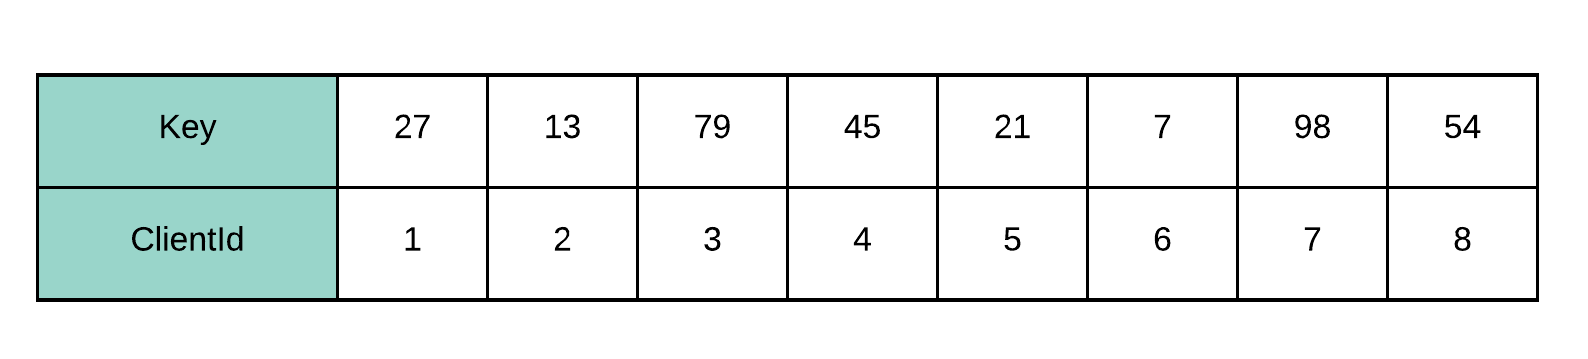
\includegraphics[width=8cm]{RandomKeysInicializado}
	\label{fig:RandomKeysInicializado2}
\end{figure}

\begin{figure}[h]
	%\caption{Vector de enteros aleatorios ordenado.}
	\centering
	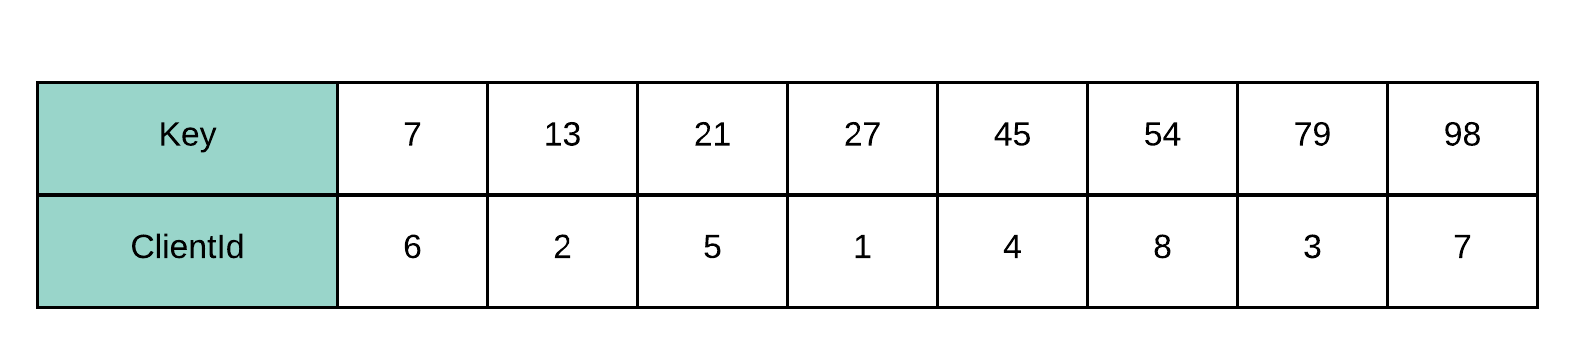
\includegraphics[width=8cm]{RandomKeysOrdenado}
	\label{fig:RandomKeysOrdenado2}
\end{figure}

\begin{itemize}
    \pause
    \item Hash resultante del vector de enteros de la imagen: 6@2@5@1@4@8@3@7
\end{itemize}

\end{frame}

%%%%%%%%%%%%%%%%%%%%%%%%%%%%%%%%%%%%%%%%%%%%%%

\begin{frame}
\frametitle{Método óptimo para calcular el hash}

\begin{itemize}
    \item Se toman los recorridos de los vehículos y se los ordena por el identificador del primer cliente que visitan. 
    \pause
    \item Se calcula el hash de cada vehículo y se concatenan utilizando otro símbolo separador.
    \pause
\end{itemize}

\begin{figure}[h]
	\caption{Vector de enteros aleatorios ordenado y la solución en la que decodifica.}
	\centering
	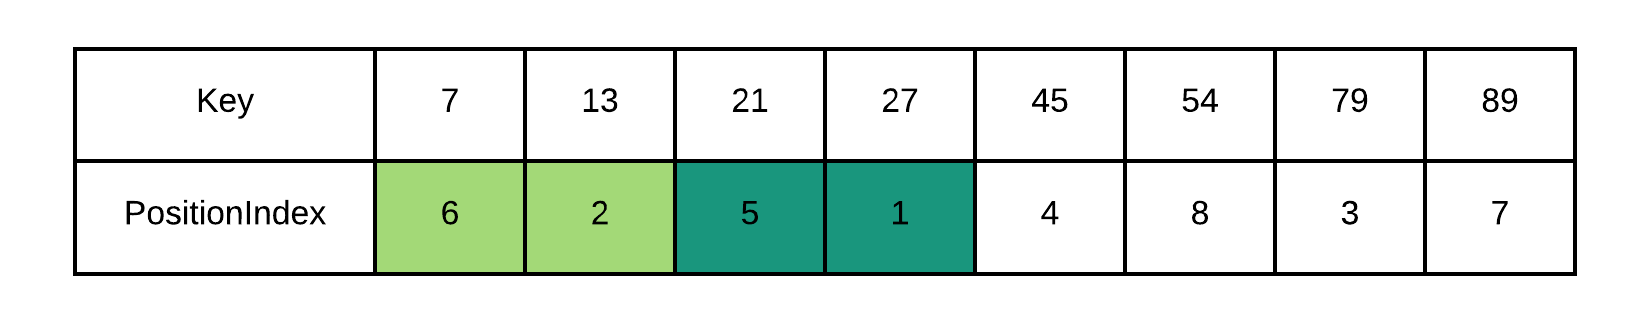
\includegraphics[width=8cm]{DistribucionClientesDecoSimple}
	\label{fig:DistribucionClientesDecoSimple2}
\end{figure}

\begin{itemize}
    \pause
    \item Hash resultante de la solución de la imagen: 5@1\#6@2
    \pause
    \item Si cambiamos la posición de los ClientId 8, 3 y 7 obtenemos la misma solución al decodificarla. El hash con este método no cambia y el hash con el método anterior cambia.
\end{itemize}

\end{frame}

%%%%%%%%%%%%%%%%%%%%%%%%%%%%%%%%%%%%%%%%%%%%%%

\subsection{Pruebas sobre el BRKGA sin búsqueda local}

\begin{frame}
\frametitle{Pruebas sobre el BRKGA sin búsqueda local}

\begin{itemize}
    \item Se realizaron varias pruebas sobre el BRKGA modificando las variables de su configuración. Tales variables:
    \pause
    \item Iteraciones. (Entre 200 y 300).
    \pause
    \item Cantidad de iteraciones sin cambios en la mejor solución. (Entre 50 y 100).
    \pause
    \item Tamaño de la población. (Entre 100 y 200).
    \pause
    \item Porcentaje de la población elite. (Entre el 20\% y el 30\%)
    \pause
    \item Porcentaje de mutantes. (Entre el 5\% y el 10\%)
    \pause
    \item Probabilidad de heredar alelo del padre elite ($\rho_e \in [0.5,0.7]$)
    \pause
    \item Tipo de decodificador. (El simple o el goloso).
\end{itemize}

\end{frame}

%%%%%%%%%%%%%%%%%%%%%%%%%%%%%%%%%%%%%%%%%%%%%%

\begin{frame}
\frametitle{La configuración que mejor resulto para el BRKGA sin Búsqueda Local}

\begin{itemize}
    \item Luego de varias pruebas, evaluando los resultados obtenidos y el tiempo de ejecución, la configuración que obtuvo los mejores resultados:
    \pause
    \item Iteraciones: 250; Sin cambios: 50; Población.100; Porcentaje elite: 30\%; Porcentaje mutante: 10\%; $\rho_e$: 0.70; Deco: Goloso.
    \pause
    \item La tabla muestra los resultados de 10 ejecuciones por instancia.
\end{itemize}

\begin{table}
\begin{center}
\begin{tabular}{ |c|c|c|c|c|c|c|c|c| } 
\hline
Instancia & N/V/D& $B_{min}$ & $B_{avg}$ & $B_{max}$ & $i_{eAvg}$ & $i_{eMax}$ & $Best$ \\
\hline
p2.2.k & 21/2/22.50 & 240 & 253 & 260 & 0.92 & 0.95 & 275 \\
p2.3.g & 21/3/10.70 & 145 & 145 & 145 & 1.00 & 1.00 & 145 \\
p3.4.p & 33/4/22.50 & 420 & 435 & 450 & 0.78 & 0.80 & 560 \\
p5.3.x & 66/3/40.00 & 735 & 735 & 735 & 0.47 & 0.47 & 1555 \\
p7.2.e & 102/2/50.00 & 200 & 209 & 222 & 0.72 & 0.77 & 290 \\
p7.4.t & 102/4/100.00 & 461 & 478 & 505 & 0.44 & 0.47 & 1077 \\
\hline
\end{tabular}
\end{center}
\label{tab:resultadosBrkgaSinBL}
\end{table}

\end{frame}

%%%%%%%%%%%%%%%%%%%%%%%%%%%%%%%%%%%%%%%%%%%%%%

\subsection{Búsqueda local}

\begin{frame}
\frametitle{Flow chart del BRKGA con búsqueda local}

\begin{figure}[h]
	\centering
	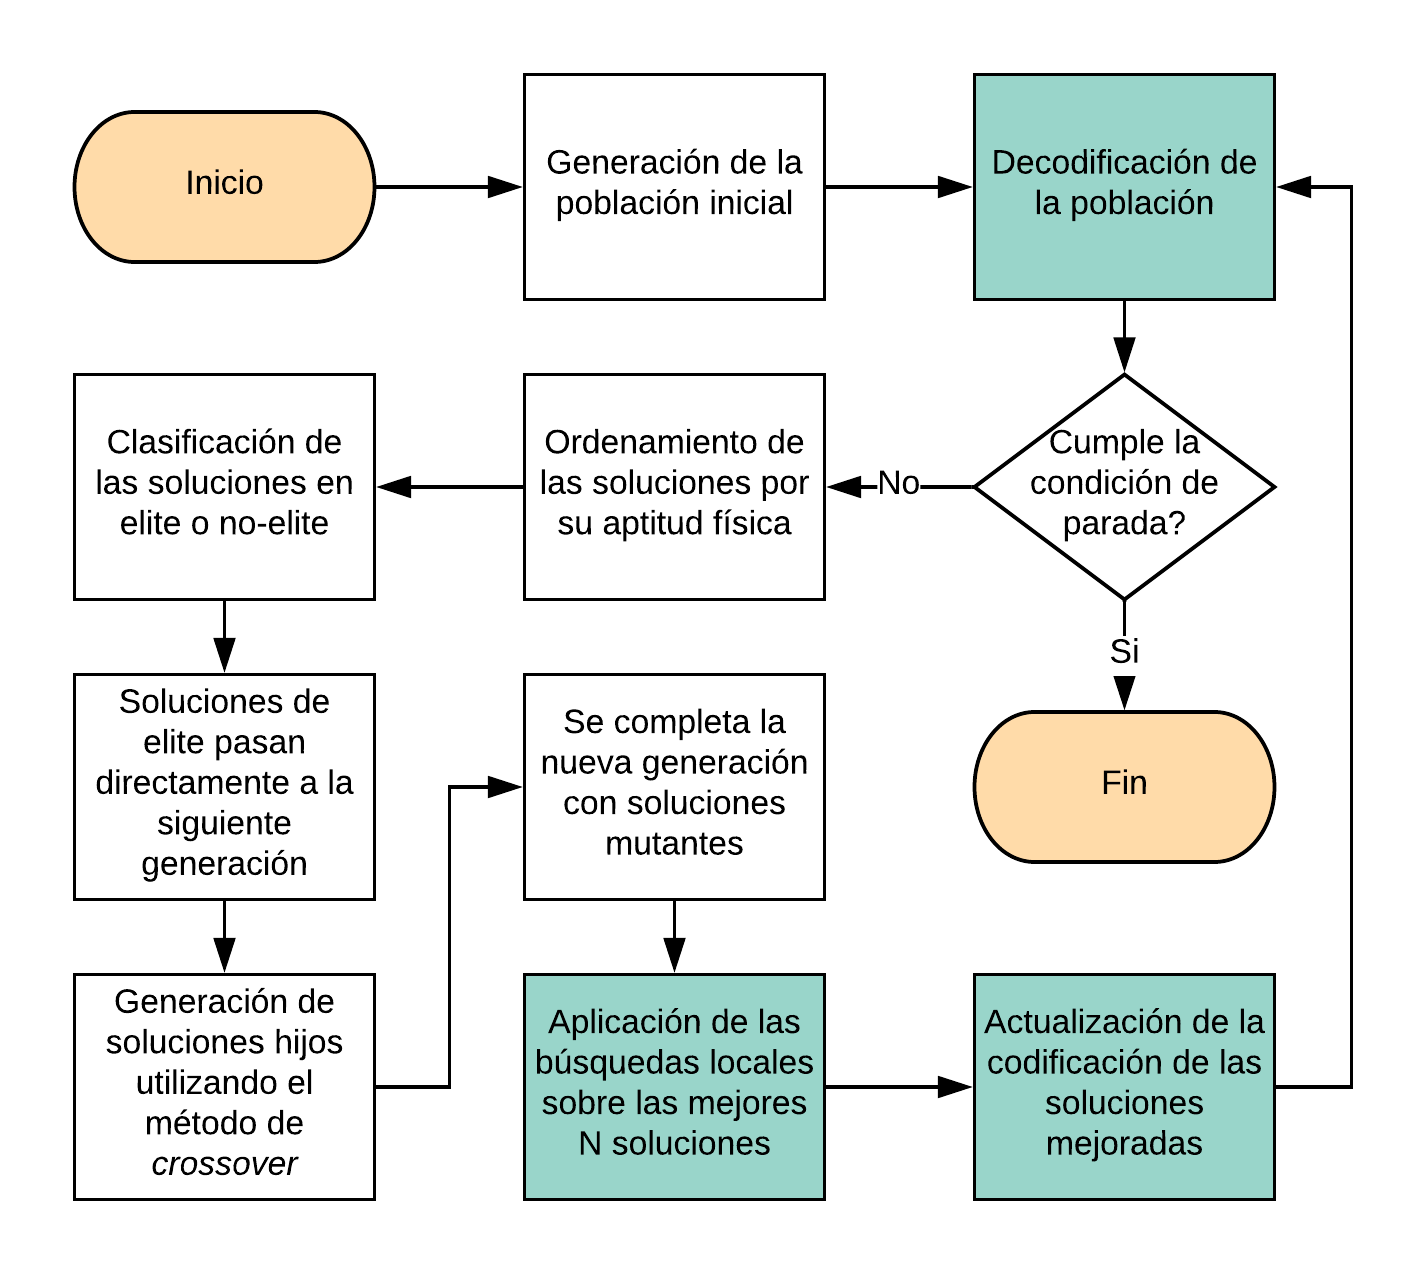
\includegraphics[width=8cm]{BRKGA_Flow_Chart_Implementado}
	\label{fig:BRKGA_Flow_Chart_Implementado}
\end{figure}

\end{frame}

%%%%%%%%%%%%%%%%%%%%%%%%%%%%%%%%%%%%%%%%%%%%%%

\begin{frame}
\frametitle{Búsqueda local: Swap}

\begin{itemize}
    \item Dados dos vehículos, busca intercambiar clientes entre sus rutas con el objetivo de reducir la suma de las distancias recorridas por ambos vehículos.
\end{itemize}

\begin{figure}[h]
	\centering
	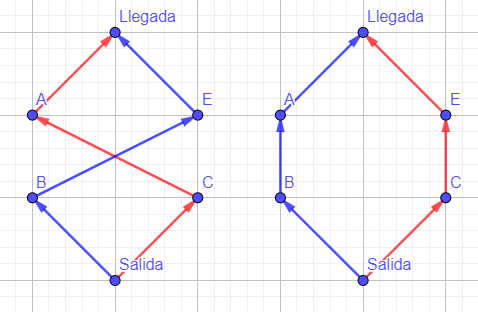
\includegraphics[width=8cm]{blswap}
	\label{fig:blswap}
\end{figure}

\end{frame}

%%%%%%%%%%%%%%%%%%%%%%%%%%%%%%%%%%%%%%%%%%%%%%

\begin{frame}
\frametitle{Búsqueda local: 2-Opt}

\begin{itemize}
    \item Dado un vehículo, cambia el orden de los clientes visitados con el objetivo de reducir la distancia recorrida.
\end{itemize}

\begin{figure}[h]
	\centering
	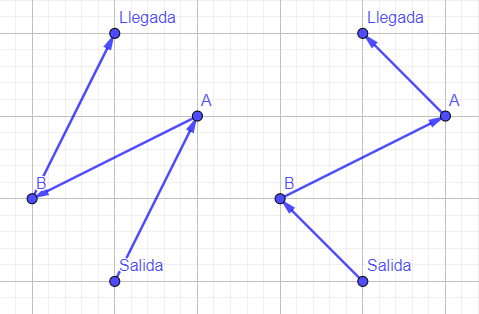
\includegraphics[width=8cm]{bl2opt}
	\label{fig:bl2opt}
\end{figure}

\end{frame}

%%%%%%%%%%%%%%%%%%%%%%%%%%%%%%%%%%%%%%%%%%%%%%

\begin{frame}
\frametitle{Búsqueda local: Insert}

\begin{itemize}
    \item Intenta insertar un cliente no visitado en la ruta de un vehículo.
\end{itemize}

\begin{figure}[h]
	\centering
	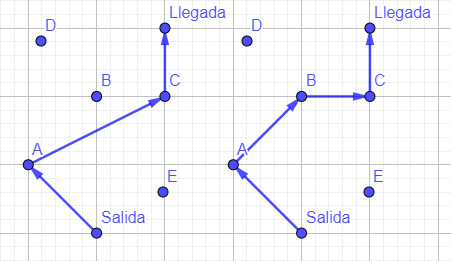
\includegraphics[width=9cm]{blinsert}
	\label{fig:blinsert}
\end{figure}

\end{frame}

%%%%%%%%%%%%%%%%%%%%%%%%%%%%%%%%%%%%%%%%%%%%%%

\begin{frame}
\frametitle{Búsqueda local: Replace Simple}

\begin{itemize}
    \item Dado un vehículo, intenta reemplazar un cliente visitado por un cliente no visitado en su ruta.
\end{itemize}

\begin{figure}[h]
	\centering
	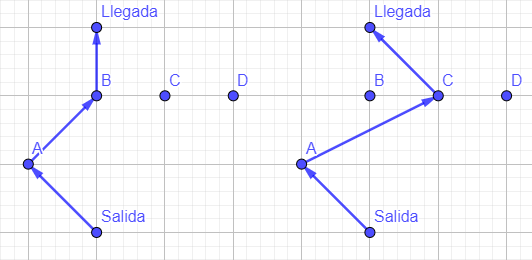
\includegraphics[width=9cm]{blreplaceSimple}
	\label{fig:blreplaceSimple}
\end{figure}

\end{frame}

%%%%%%%%%%%%%%%%%%%%%%%%%%%%%%%%%%%%%%%%%%%%%%

\begin{frame}
\frametitle{Búsqueda local: Replace Multiple}

\begin{itemize}
    \item Dado un vehículo, intenta reemplazar uno o varios clientes visitados por un cliente no visitado en su ruta.
\end{itemize}

\begin{figure}[h]
	\centering
	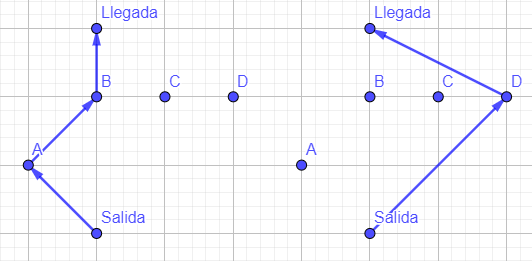
\includegraphics[width=9cm]{blreplaceMultiple}
	\label{fig:blreplaceMultiple}
\end{figure}

\end{frame}

%%%%%%%%%%%%%%%%%%%%%%%%%%%%%%%%%%%%%%%%%%%%%%

\subsection{Centro de gravedad}

\begin{frame}
\frametitle{Centro de gravedad (COG)}

\begin{itemize}
    \item En las búsquedas locales que buscan clientes candidatos a agregar entre los no visitados, se priorizan aquellos más cercanos al centro de gravedad de la ruta.
    \pause 
    \item El COG es un punto en el plano, por lo tanto, tiene una coordenada $x$ y una coordenada $y$.
    \pause 
    \item La coordenada $x_{COG}$ es el promedio de todas las coordenadas $x$ de los clientes de la ruta ponderados por el beneficio del cliente. (Idem $y_{COG}$).
    \pause 
    \item $x_{cog} = (\sum_{\forall i \in ruta} x_i * B_i) / \sum_{\forall i \in ruta} B_i$
    \pause 
    \item $y_{cog} = (\sum_{\forall i \in ruta} y_i * B_i) / \sum_{\forall i \in ruta} B_i$
\end{itemize}

\end{frame}

%%%%%%%%%%%%%%%%%%%%%%%%%%%%%%%%%%%%%%%%%%%%%%

\begin{frame}
\frametitle{Centro de gravedad (COG)}

\begin{itemize}
    \item La figura muestra el centro de gravedad asumiendo que todos los clientes en la ruta tienen el mismo beneficio. Orden de los clientes según su cercanía al COG: $c_7$, $c_5$, $c_8$ y $c_6$.
\end{itemize}

\begin{figure}[h]
	\centering
	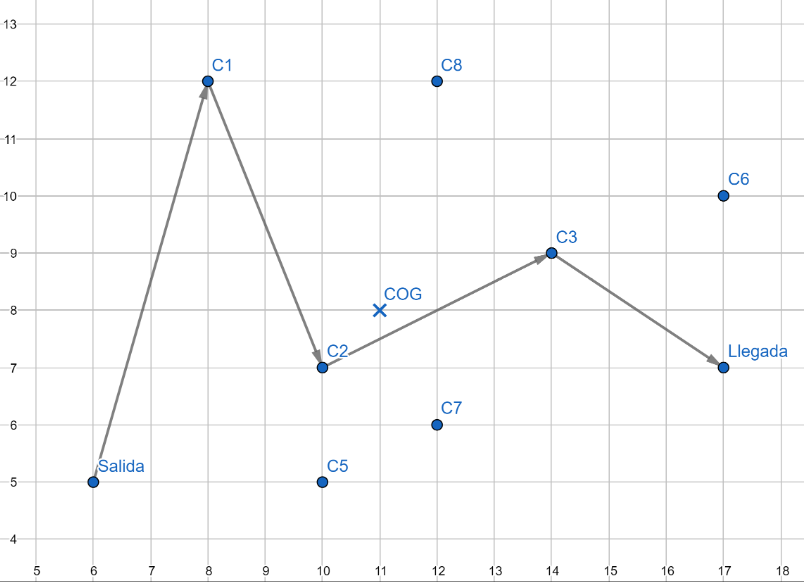
\includegraphics[width=9cm]{COG}
	\label{fig:COG}
\end{figure}

\end{frame}

%%%%%%%%%%%%%%%%%%%%%%%%%%%%%%%%%%%%%%%%%%%%%%

\subsection{Codificación de las soluciones}

\begin{frame}
\frametitle{Codificación de las soluciones mejoradas}

\begin{itemize}
    \item Una vez que se modifican las soluciones, debemos actualizar su codificación de modo tal que al decodificarla obtengamos la solución mejorada en vez de su versión anterior.
    \pause
    \item Si no actualizamos su codificación (vector de enteros aleatorios), cuando se utilice la solución mejorada como padre en el \textit{crossover} sus características viejas serán las que heredará la solución resultante.
    \pause
\end{itemize}

\begin{figure}[h]
	\centering
	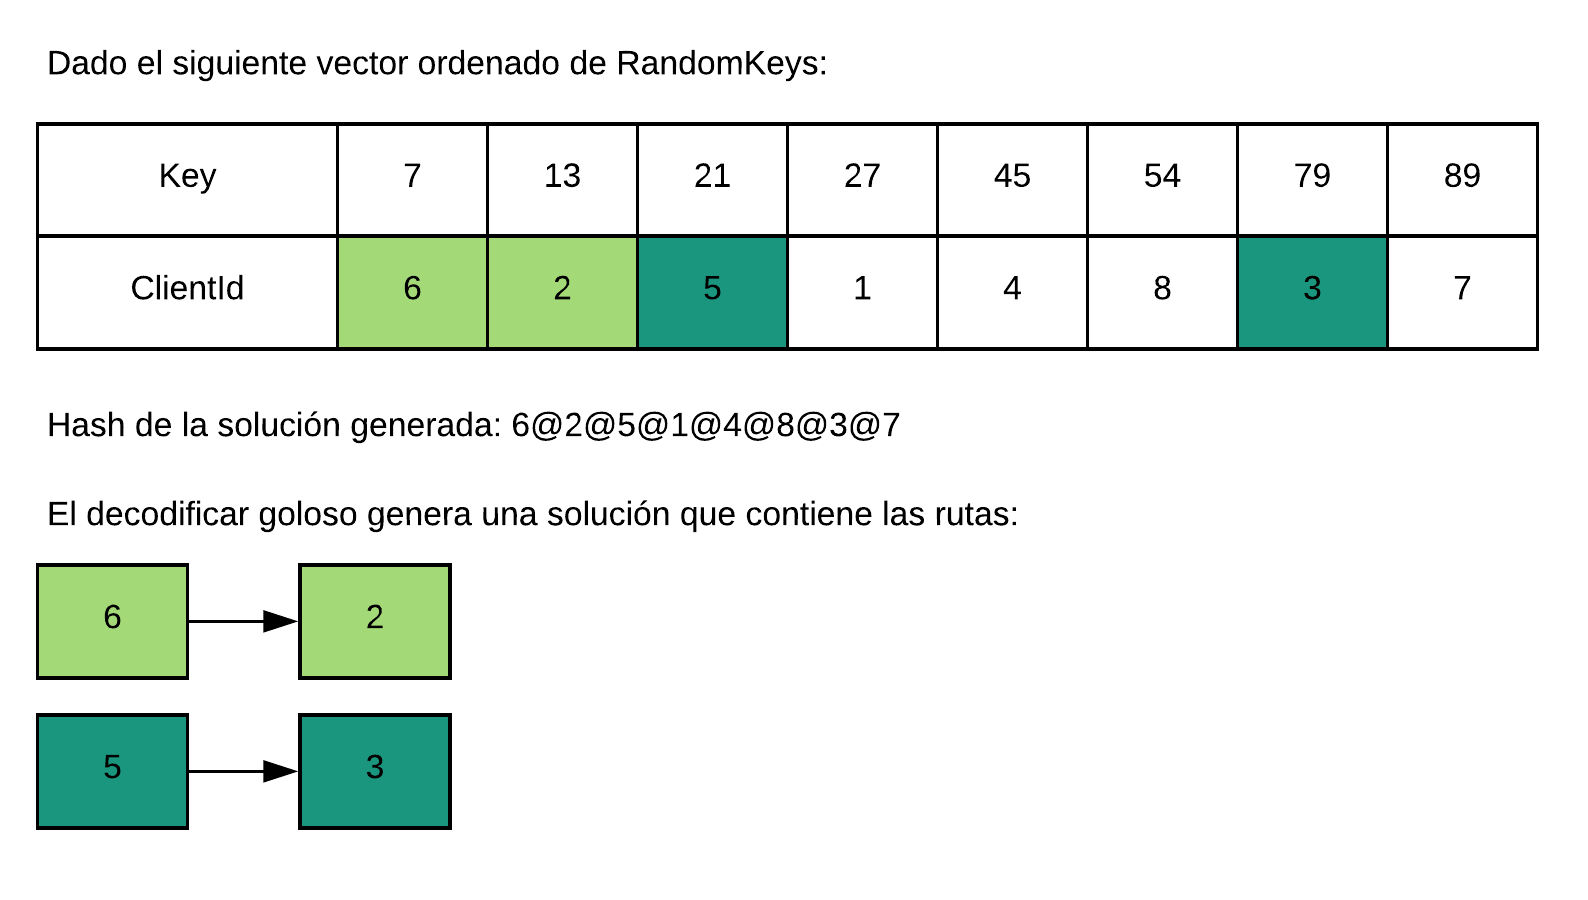
\includegraphics[width=8cm]{codificacionDeSolucionParteUno}
	\label{fig:codificacionDeSolucionParteUno}
\end{figure}

\end{frame}

%%%%%%%%%%%%%%%%%%%%%%%%%%%%%%%%%%%%%%%%%%%%%%

\begin{frame}
\frametitle{Codificación de las soluciones mejoradas}

\begin{figure}[h]
	\centering
	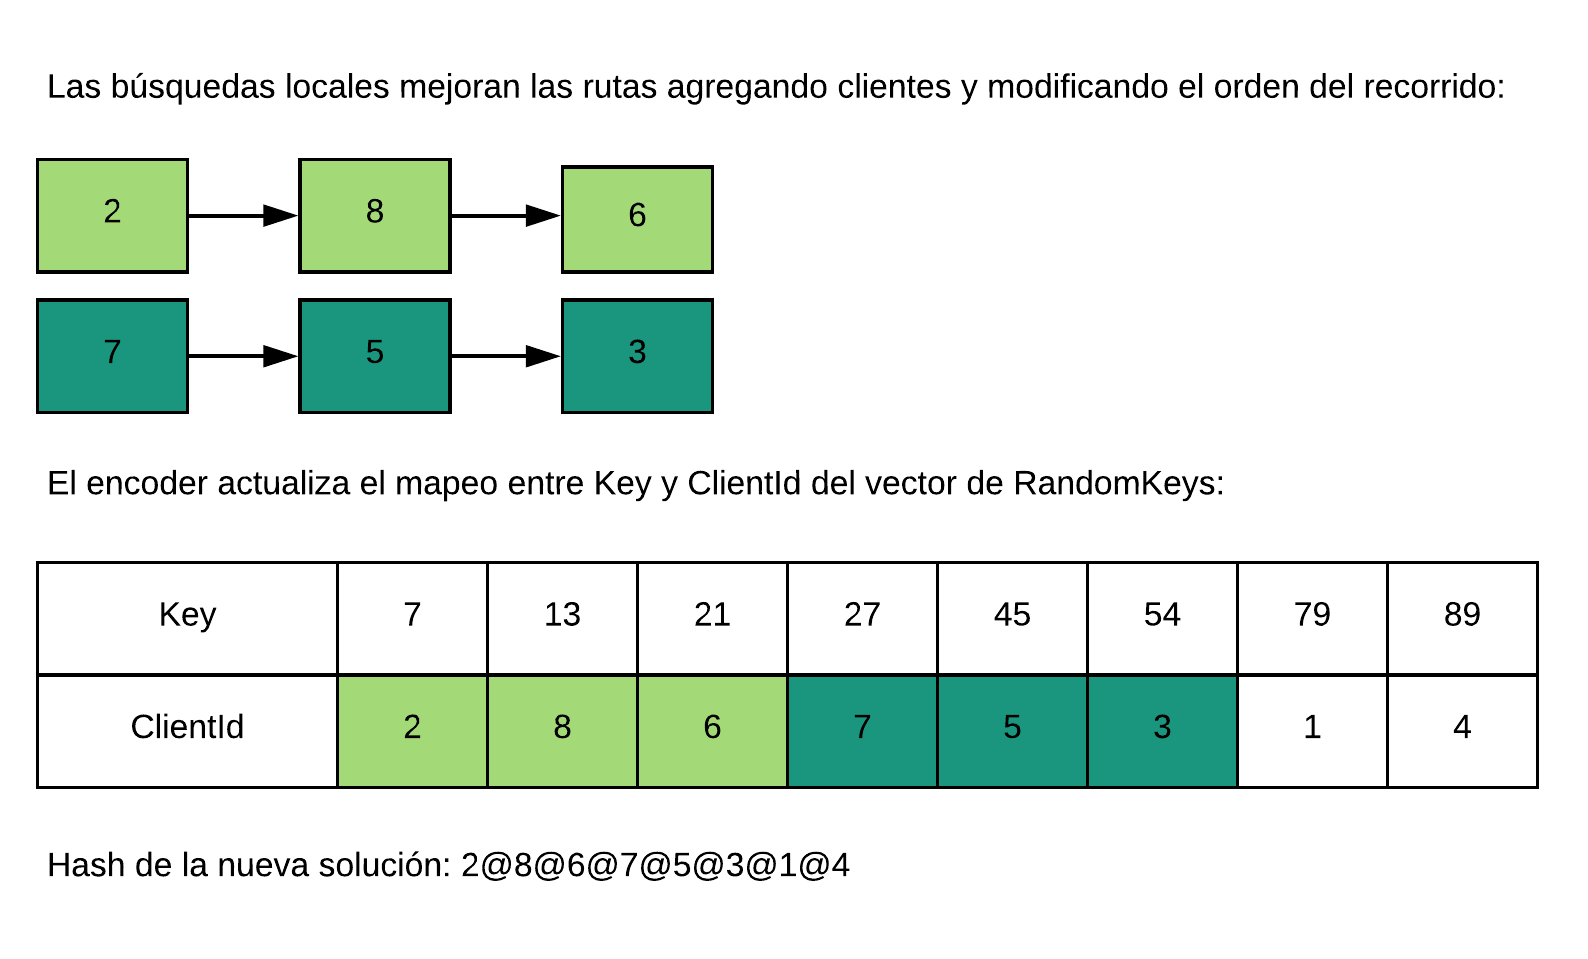
\includegraphics[width=8cm]{codificacionDeSolucionParteDos}
	\label{fig:codificacionDeSolucionParteDos}
\end{figure}

\begin{itemize}
    \item En la figura podemos ver que no se modificaron los \textit{keys} ni los \textit{ClientId}, lo que se modificó fueron las asociaciones entre ellos. De forma tal que cuando se ordena el vector de enteros aleatorios según los \textit{keys}, obtenemos los clientes ordenados por vehículo y luego el orden en que serán visitados.
\end{itemize}

\end{frame}

%%%%%%%%%%%%%%%%%%%%%%%%%%%%%%%%%%%%%%%%%%%%%%

\subsection{Orden en que se aplican las búsquedas locales}

\begin{frame}
\frametitle{Orden en que se aplican las búsquedas locales}

\begin{itemize}
    \item En cada nueva generación se le aplican las búsquedas locales a la mejor solución (que no haya sido mejorada en una generación anterior).
    \pause
    \item El orden en que se aplican las estrategias de búsqueda local es importante.
    \pause
    \item Por ejemplo, el \textit{2-Opt} busca reducir la distancia recorrida de un vehículo. Por lo tanto, si aplicamos el \textit{2-Opt} al final, no hacemos uso de la distancia ahorrada y la aptitud de la solución resultante no incrementa.
    \pause
    \item Realicé varias pruebas modificando el orden en que se aplican las búsquedas locales, medí sus tiempos y los resultados finales.
    \pause
    \item Para tales pruebas mantuve constante el resto de la configuración del BRKGA de modo que no influya en el resultado.
\end{itemize}

\end{frame}

%%%%%%%%%%%%%%%%%%%%%%%%%%%%%%%%%%%%%%%%%%%%%%

\begin{frame}
\frametitle{Orden en que se aplican las búsquedas locales}

\begin{itemize}
    \item Siglas de las búsquedas locales.
    \pause
    \item Swap: \textbf{S}
    \pause
    \item 2-Opt: \textbf{O}
    \pause
    \item Insert: \textbf{I}
    \pause
    \item Replace Simple: \textbf{Rs}
    \pause
    \item Replace Múltiple: \textbf{Rm}
    \pause
    \item Por lo tanto, si en la fila dice \textbf{SRsOIRm} significa que las búsquedas aplicaron en el siguiente orden: Swap, Replace Simple, 2-Opt, Insert y Raplace Multiple.    
\end{itemize}

\end{frame}

%%%%%%%%%%%%%%%%%%%%%%%%%%%%%%%%%%%%%%%%%%%%%%

\begin{frame}
\frametitle{Orden en que se aplican las búsquedas locales}

\begin{itemize}
    \item Resultados de 25 ejecuciones sobre la instancia \textit{p5.3.x}. En la siguiente tabla se ven 7 posibles combinaciones de las búsquedas.
\end{itemize}

\begin{table}
\begin{center}
\begin{tabular}{ |c|c|c|c|c|c|c|c| } 
\hline
Orden BL & $T_{avg}$ & $B_{min}$ & $B_{avg}$ & $B_{max}$ & $i_{eAvg}$ & $i_{eMax}$ & $Best$ \\
\hline
IRmRsOS & 49397 & 1460 & 1485 & 1540 & 0.95 & 0.99 & 1555  \\
ORsSIRm & 39576 & 1485 & 1509 & 1525 & 0.97 & 0.98 & 1555  \\
SIORsSORm & 43556 & 1495 & 1512 & 1535 & 0.97 & 0.99 & 1555  \\
SOIORsRmSORm & 49449 & 1505 & 1522 & 1545 & 0.98 & 0.99 & 1555  \\
SOIRsRm & 36595 & 1500 & 1512 & 1525 & 0.97 & 0.98 & 1555  \\
\textbf{SOSIRsSORm} & 40375 & 1505 & 1521 & 1535 & 0.98 & 0.99 & 1555  \\
SRsOIRm & 43423 & 1480 & 1510 & 1535 & 0.97 & 0.99 & 1555  \\
\hline
\end{tabular}
\end{center}
\label{tab:resultadosListaLS1}
\end{table}

\end{frame}

%%%%%%%%%%%%%%%%%%%%%%%%%%%%%%%%%%%%%%%%%%%%%%

\begin{frame}
\frametitle{Orden en que se aplican las búsquedas locales}

\begin{itemize}
    \item Resultados de 25 ejecuciones sobre la instancia \textit{p7.4.t}. En la siguiente tabla se ven 7 posibles combinaciones de las búsquedas.
\end{itemize}

\begin{table}
\begin{center}
\begin{tabular}{ |c|c|c|c|c|c|c|c| } 
\hline
Orden BL & $T_{avg}$ & $B_{min}$ & $B_{avg}$ & $B_{max}$ & $i_{eAvg}$ & $i_{eMax}$ & $Best$ \\
\hline
IRmRsOS & 81876 & 1004 & 1038 & 1064 & 0.96 & 0.99 & 1077  \\
ORsSIRm & 86537 & 1024 & 1038 & 1063 & 0.96 & 0.99 & 1077  \\
SIORsSORm & 91839 & 1033 & 1049 & 1077 & 0.97 & 1.00 & 1077  \\
SOIORsRmSORm & 126705 & 1042 & 1055 & 1069 & 0.98 & 0.99 & 1077  \\
SOIRsRm & 82889 & 1032 & 1047 & 1071 & 0.97 & 0.99 & 1077  \\
\textbf{SOSIRsSORm} & 94731 & 1038 & 1055 & 1071 & 0.98 & 0.99 & 1077  \\
SRsOIRm & 90306 & 1024 & 1042 & 1067 & 0.97 & 0.99 & 1077  \\
\hline
\end{tabular}
\end{center}
\label{tab:resultadosListaLS2}
\end{table}

\end{frame}

%%%%%%%%%%%%%%%%%%%%%%%%%%%%%%%%%%%%%%%%%%%%%%

\section{Resultados}

\begin{frame}
\frametitle{Resultados}

Se compararon los resultados con los de los siguientes trabajos:

\begin{itemize}
	\item \textit{The team orienteering problem}. Implementaron una optimización multinivel. (CGW) Chao I-M., Golden B.L. yWasil E.A. European Journal of Operational Research, 88:464-474, (1996).
	\pause
	\item \textit{A tabu search heuristic for the team orienteering problem}. (TMH) Tang H. y Miller-Hooks E. Computers and Operations Research, 32:1379-1407, (2005).
\end{itemize}
\end{frame}

%%%%%%%%%%%%%%%%%%%%%%%%%%%%%%%%%%%%%%%%%%%%%%

\begin{frame}
\frametitle{Resultados}

\begin{itemize}
	\item \textit{Metaheuristics for the team orienteering problem}. Propusieron 2 Variable Neighborhood Search y 2 Búsquedas Tabú, los mejores resultados los obtuvieron en su VNS slow. ($VNS_{slow}$) Archetti C., Hertz A. y M.G. Speranza. Journal of Heuristics, 13:49-76, (2007).
	\pause
	\item \textit{Ants can solve the team orienteering problem}. ($ACO_{seq}$) Ke L., Archetti C. y Feng Z. Computers and Industrial Engineering, 54:648-665, (2008).
	\pause
	\item \textit{A memetic algorithm for the team orienteering problem}. (MA) Bouly H., Dang D.-C. y Moukrim A. A Quarterly Journal of Operations Research, 8:49-70, (2010).
\end{itemize}

\end{frame}

%%%%%%%%%%%%%%%%%%%%%%%%%%%%%%%%%%%%%%%%%%%%%%

\begin{frame}
\frametitle{Resultados}

\begin{itemize}
    \item Se ejecutó 3 veces la versión final sobre cada una de las 345 instancias del benchmarck.
    \pause
    \item La tabla muestra el resultado para 6 instancias representativas del benchmark.
\end{itemize}

\begin{table}
\begin{center}
\begin{tabular}{ |c|c|c|c|c|c|c|c| } 
\hline
Instancia & N/V/D & $B_{min}$ & $B_{avg}$ & $B_{max}$ & $i_{eAvg}$ & $i_{eMax}$ & $Best$ \\
\hline
p2.2.k & 21/2/22.50 & 270 & 274 & 275 & 1.00 & 1.00 & 275 \\
p2.3.g & 21/3/10.70 & 145 & 145 & 145 & 1.00 & 1.00 & 145 \\
p3.4.p & 33/4/22.50 & 560 & 560 & 560 & 1.00 & 1.00 & 560 \\
p5.3.x & 66/3/40.00 & 1515 & 1524 & 1550 & 0.98 & 1.00 & 1555 \\
p7.2.e & 102/2/50.00 & 290 & 290 & 290 & 1.00 & 1.00 & 290 \\
p7.4.t & 102/4/100.00 & 1047 & 1054 & 1064 & 0.98 & 0.99 & 1077 \\
\hline
\end{tabular}
\end{center}
\label{tab:resultados}
\end{table}

\end{frame}

%%%%%%%%%%%%%%%%%%%%%%%%%%%%%%%%%%%%%%%%%%%%%%

\begin{frame}
\frametitle{Resultados}

\begin{itemize}
    \item $\delta Z_{min} = \sum_{i \in instance} Best_i - B_{min}$
    \pause
    \item $\delta Z_{max} = \sum_{i \in instance} Best_i - B_{max}$
    \pause
    \item $\delta Z = \delta Z_{min} - \delta Z_{max}$
    \pause
\end{itemize}

\begin{table}
\begin{center}
\begin{tabular}{ |c|c|c|c|c|c|c|c|c| } 
\hline
Algoritmo & $\delta Z_{min}$ & $\delta Z_{max}$ & $\delta Z$  \\
\hline
CGW & 4340 & - & -  \\
BRKGA\textsubscript{bl} & 3054 & 1636 & 1418  \\
TMH & 2404 & - & -  \\
TS\textsubscript{penalty} & 2376 & 981 & 1395  \\
TS\textsubscript{feasible} & 1184 & 399 & 785  \\
VNS\textsubscript{fast} & 1436 & 352 & 1084  \\
VNS\textsubscript{slow} & 427 & 84 & 343  \\
ACO\textsubscript{seq} & - & 204 & -  \\
MA & 434 & 80 & 354  \\
\hline
\end{tabular}
\end{center}
%\caption{Síntesis de los resultados.}
\label{tab:resultadosSintesis}
\end{table}

\end{frame}

%%%%%%%%%%%%%%%%%%%%%%%%%%%%%%%%%%%%%%%%%%%%%%

\section{Conclusiones}

\begin{frame}
\frametitle{Conclusiones}

\begin{itemize}
    \item Un 70\% de los resultados llegaron a la mejor solución conocida de la instancia testeada.
    \pause
    \item El restante 30\% obtuvo valores competitivos con los mejores trabajos previos.
    \pause
    \item El BRKGA sin búsqueda local no dió buenos resultados para instancias grandes del problema.
    \pause
    \item Se implementaron variantes de decodificadores.
    \pause
    \item Se implementaron dos formas de calcular el hash para resolver el problema de individuos repetidos.
    \pause
    \item Se implementaron diversas búsquedas locales y un codificador de soluciones para mantener la consistencia entre los individuos y sus genes.
    \pause
    \item Se realizaron múltiples pruebas de eficiencia variando las configuraciones generales.
\end{itemize}

\end{frame}

%%%%%%%%%%%%%%%%%%%%%%%%%%%%%%%%%%%%%%%%%%%%%%

\section{Trabajos Futuros}

\begin{frame}
\frametitle{Trabajos Futuros}

\begin{itemize}
    \item Sería útil una herramienta para visualizar los caminos generados.
    \pause
    \item Investigar otras variantes de decodificadores. Ej, particionar los clientes según su centro de gravedad, asignar un vehículo a cada centro y seleccionar un orden de clientes por centro de gravedad según un vector de enteros aleatorios.
    \pause
    \item Investigar otros métodos de \textit{crossover}. Ej, Que cada alelo represente un vehículo con su ruta en vez de un cliente.
    \pause
    \item Analizar si existe alguna otra variante del BRKGA que genere buenos resultados sin depender de las búsquedas locales.
\end{itemize}

\end{frame}

%%%%%%%%%%%%%%%%%%%%%%%%%%%%%%%%%%%%%%%%%%%%%%

%------------------------------------------------

\begin{frame}
\Huge{\centerline{Gracias!}}
\end{frame}

%----------------------------------------------------------------------------------------

\end{document} 